\section{引\quad 言}
火星探测器气动捕获的整体制动过程如图\ref{figIntroSketch}所示。
\begin{center}
	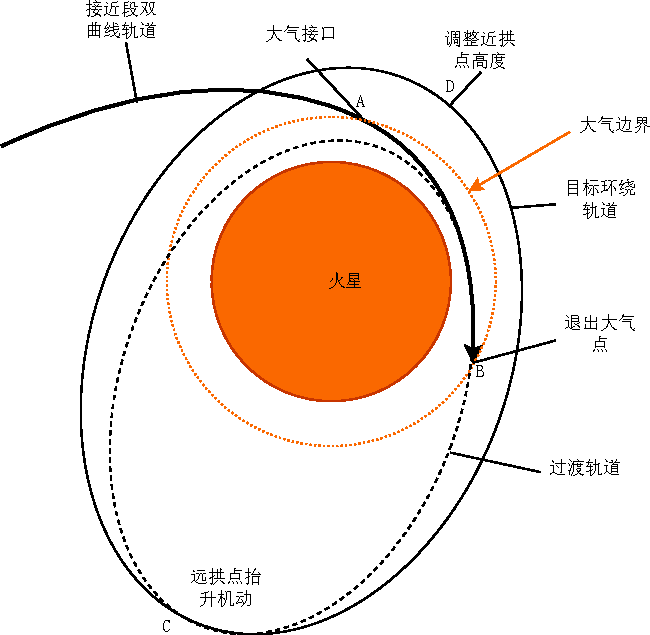
\includegraphics[scale=0.8]{IntroSketch.pdf}  \\
	\figcaption{被控对象模型的模块框图} \label{figIntroSketch}
\end{center}
飞行器首先由$A$点沿双曲线轨道进入火星大气,从$A$到$B$点为气动飞行轨道段,气动捕获制导的任务就是在此期间通过改变控制量利用气动力实现减速,当 飞行器从 B 点飞出大气后需要形成环绕轨道,若 AB 段气动捕获任务不成功,飞 行器将继续沿某条双曲线轨道飞离火星,或飞行器没有飞出大气层,直接撞向火 星地面,以上任意两种情形发生都会直接导致失败。成功环绕后所形成的椭圆轨 道称为过渡轨道,图中用虚线表示,该轨道的近点位于火星大气范围内。若此后 需要形成围绕火星进行探测的停泊轨道,则需要当飞行器沿过渡轨道飞至远拱点 时(图中 C 点)需要进行点火制动,将近拱点抬升出大气影响范围;若此后需要 直接进行下降着陆任务,则不需要此项制动,或仅需进行轨道微调但不需将近点 抬出大气。当飞行器再次抵近拱点时(图中 D 点),可再次进行轨道机动对远拱点 进行调整。
气动捕获制导的总体思路是,
通过不断预测以当前控制量飞出大气后的过渡轨道状态向量与目标轨道的状态向量间的误差,
代入制导算法来产生新的控制量,
如此往复,直到满足终端需求为止。

气动捕获采用倾侧角作为控制量而不是攻角的原因是,
攻角幅度过大会影响飞行器的热控能力。
